\section{Implementation Details}
\label{sec:implementation}

We design CodFS based on commodity configurations. We implement all the
components including the client and the storage backend in C++ on Linux.
CodFS leverages several third-party libraries for high-performance operations,
including: (1) Threadpool \cite{boosttp}, which manages a pool of threads that
parallelize I/O and encoding operations, (2) Google Protocol Buffers
\cite{protobuf}, which serialize message communications between different
entities, (3) Jerasure \cite{plank09}, which provides interfaces for
efficient erasure coding implementation, and (4) FUSE \cite{fuse}, which
provides a file system interface for clients.

\begin{figure}[t]
 \centering
 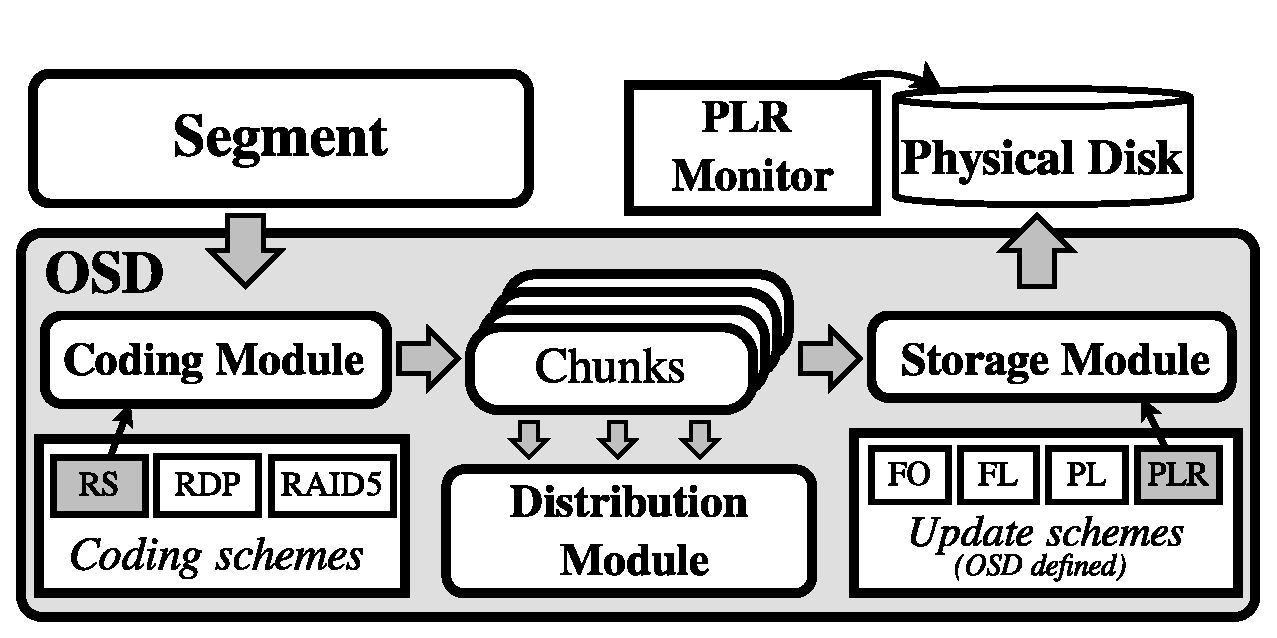
\includegraphics[width=0.7\linewidth]{figs/osd_implement}
 \caption{Internals of an OSD.}
 \label{fig:osd_implement}
\end{figure}

Figure~\ref{fig:osd_implement} illustrates the OSD design. 
We design the OSD via a modular approach. The \textit{Coding Module} of 
each OSD provides a standard interface for implementation of different coding
schemes.  One can readily extend CodFS to support new coding schemes.
The \textit{Storage Module} inside each OSD acts as an abstract layer between
the physical disk and the OSD process.  We store chunk updates and parity
deltas according to the update scheme configured in the \textit{Storage
Module}.  By default, CodFS uses the \PLR scheme. Each OSD is equipped with
a \textit{Monitor Module} to perform garbage collection in \FL and \PL and
reserved space shrinking and prediction in \PLR.

We adopt Linux Ext4 as the local filesystem of each OSD to support fast
reserved space allocation.  We pre-allocate the reserved space for each parity
chunk using the Linux system call \texttt{fallocate}, which marks the
allocated blocks as uninitialized. 
%which does not require writing zero in advance. 
Shrinking of the reserved space is implemented by invoking \texttt{fallocate}
with the \texttt{FALLOC\char`_FL\char`_\\PUNCH\char`_HOLE} flag. Since we
allocate or shrink the reserved space as a multiple of chunk size, we avoid
creating unusable holes in the file system.
%and we will evaluate the three strategies in \S\ref{sec:reserve_evaluation}. 

%Our prototype currently does not address consistency and
%garbage collection of the log-structured design, and we pose their performance
%issues as future work.

%We also build a file system interface in the CodFS client using FUSE
%\cite{fuse}. 

%Apart from the native CodFS client program, we also provide a FUSE \cite{fuse}
%client implementation such that traditional file system benchmark tools could
%be used to compare CodFS with existing file systems.
%from scratch in 25,000 lines of C++ code and test on Ubuntu 12.04. 
%We also include several third-party libraries in CodFS for high performance.  
%development and testing of commonly adopted
%techniques. (1) Boost Threadpool \cite{boosttp} is used to facilitate the
%extensive use of multi-threading in CodFS. (2) Google Protocol Buffers
%\cite{protobuf} is used to serialize protocols between components. (3) Jerasure
%Library \cite{plank07} is used to perform erasure coding in CodFS.
% Reset caption spacing 

